\chapter{Comparison between the MENP framework and the traditional hypothesis testing framework}
Chapter 4 showed that the MENP framework can be applied to spectrum sensing to achieve the largest probability of detection under any possible probability of false alarm constraints. This chapter conducts a comparison between the MNEP framework and the traditional hypothesis testing framework when applied to energy detector in the presence of two primary signals. Two situations, one assuming the detector has no side information of primary users (for a given time slot, the detector does not know which primary signal could occupy the channel) and the other assuming the detector has perfect side information of primary users (for a given time slot, the detector knows which primary user could occupy the channel), are considered.  
Performance analysis results, which illustrate the performance of both framework, are presented.

\section{Energy Detection with no Side Information}
\subsection{System Model}
We consider a cognitive radio system where the licensed frequency spectrum could be occupied by one of two distinct signals $\{s_A, s_B\}$ or it could be vacant. 
Let $H_0$ denote the hypothesis under which the channel is free, $H_1$ denote the hypothesis under which the channel is occupied by $s_A$ or $s_B$.
Under hypothesis $H_1$, the channel is occupied by signal $s_A$ with probability $q$ and the channel is occupied by signal $s_B$ with probability $1-q$. %However, the value of $q$ is unknown for the detector.   
We are interested to test $H_0$ against $\bar{H}_0$. The block diagram of the system is illustrated in Figure \ref{pic: ch5 disgram}.  

\begin{figure}[!hbp]
\centering
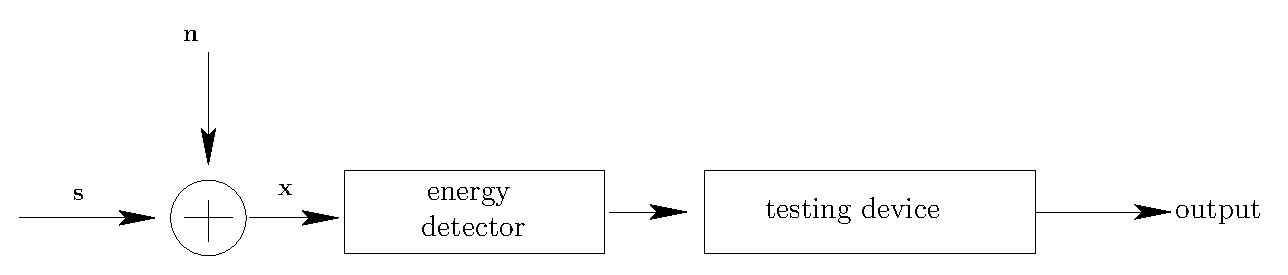
\includegraphics[width = \textwidth]{5/fig4.eps}
\caption{Block Diagram for Energy Detection}
\label{pic: ch5 diagram}
\end{figure}

The detector consists of a measuring device followed by a testing device. The measuring device observes the noises version of the received signals and forms the energy of their sampled version. With this energy, the testing device employs a proper hypothesis testing framework to decide about the state of the channel. We assume during the detection, the channel status does not change. The input to the measuring device is  
\begin{eqnarray}
  \mathbf{x} = \begin{cases}
    &\mathbf{n}\;\;\;\;\;\;\text{when $H_0$ is true}\\
    &\mathbf{n} + T\mathbf{s}_A + (1-T)\mathbf{s}_B\;\;\;\;\;\;\text{when $H_1$ is true}
  \end{cases}
  \label{equ:input2energy}
\end{eqnarray}
where
\begin{equation}
  \begin{cases}
	&\mathbf{x} = (x_0, x_1, \cdots, x_{N-1})\\
	&\mathbf{s}_A = (s_{A0}, s_{A1}, \cdots, s_{A(N-1)})\\
	&\mathbf{s}_B = (s_{B0}, s_{B1}, \cdots, s_{B(N-1)})\\
	&\mathbf{n} = (n_{0}, n_{1}, \cdots, n_{N-1})\,,
  \end{cases}
  \label{150621a1}
\end{equation}
and 
\begin{equation}
  T = \begin{cases}
    &0\;\;\;\;\;\;\text{with probability $q$}\\
    &1\;\;\;\;\;\;\text{with probability $1-q$}\,.
  \end{cases}
  \label{150621a2}
\end{equation}

Just like in section 4.1, 
we assume  $s_{A_i}$ $s_{B_i}$ and $n_i$ are zero-mean independent and identically distributed (iid) circularly symmetric complex Gaussian (CSCG) random variables with variances $2\sigma_{s_A}^2$, $2\sigma_{s_B}^2$ and $2\sigma_{n}^2$, i.e., $s_{A_i} \sim \mathcal{CN}(0, 2\sigma_{s_A}^2)$, $s_{B_i} \sim \mathcal{CN}(0, 2\sigma_{s_B}^2)$ and $n_i \sim \mathcal{CN}(0, 2\sigma_{n}^2)$.
Each noisy sample $x_i = s_i + n_i$ is governed by a probability law under each hypothesis. In our model
since the noise and signal are independent, $s_i+ n_i \sim \mathcal{CN}(0, 2(\sigma_{s}^2 + \sigma_n^2))$.  Define $\sigma_0^2 = \sigma_n^2$, $\sigma_1^2 = \sigma_{s_A}^2 + \sigma_n^2$ and $\sigma_2^2 = \sigma_{s_B}^2 + \sigma_n^2$, we can see
\begin{equation}
  \label{1129a1}
  \begin{split}
  n_i &\sim \mathcal{CN}(0, 2\sigma_0^2)\\
  n_i + s_{A_i} &\sim \mathcal{CN}(0, 2\sigma_1^2)\\
   n_i + s_{B_i}&\sim \mathcal{CN}(0, 2\sigma_2^2) \,,
  \end{split}
\end{equation}
thus we have 

\begin{equation}
   \begin{split}
     \begin{pmatrix} x_{i_R} \\ x_{i_I} \end{pmatrix} \sim \mathcal{N}\Big( \begin{bmatrix} 0 \\ 0 \end{bmatrix}, \begin{bmatrix} \sigma_0^2 & 0\\ 0 & \sigma_0^2 \end{bmatrix} \Big) \text{when no signal is presented}\\
     \begin{pmatrix} x_{i_R} \\ x_{i_I} \end{pmatrix} \sim \mathcal{N}\Big( \begin{bmatrix} 0 \\ 0 \end{bmatrix}, \begin{bmatrix} \sigma_1^2 & 0\\ 0 & \sigma_1^2 \end{bmatrix} \Big) \text{when $s_A$ is presented}\\
     \begin{pmatrix} x_{i_R} \\ x_{i_I} \end{pmatrix} \sim \mathcal{N}\Big( \begin{bmatrix} 0 \\ 0 \end{bmatrix}, \begin{bmatrix} \sigma_2^2 & 0\\ 0 & \sigma_2^2 \end{bmatrix} \Big) \text{when $s_B$ is presented}
\end{split}
  \label{equ:xdistribution2}
\end{equation}
where $x_{i_R}$ and $x_{i_I}$ are real and imaginary components of $x_i$. Like in section 4.1, the output of measuring device is

\begin{equation} 
  Y = \sum_{i=0}^{N-1}|x_i|^2 = \sum_{i=0}^{N-1}(x_{i_R}^2+x_{i_I}^2)\,.
  \label{equ: testing device2}
\end{equation}
By observing $y$, a realization of $Y$, the testing device determines the status of the channel. As we have shown in section 3.1 and section 4.1, when the frequency channel is ideal, the distribution of $Y$ can be written as
\def \CHISQUY[#1]{\frac{1}{#1 2^N\Gamma(N)}\left(\frac{y}{#1}\right)^{N-1}\exp\left(-\frac{y}{2#1}\right)\\}
\begin{equation}
  f_0(y) = \CHISQU[\sigma_0^2]\,;
  \label{20150621a4}
\end{equation}
and when the channel is occupied by primary signal, according $T=1$ or $T=0$, the distribution of $Y$ can be written as, 
\begin{equation}
  f_1(y|T=1) = \CHISQU[\sigma_1^2]\,,
  \label{20150621a5}
\end{equation}
\begin{equation}
  f_1(y|T=0) = \CHISQU[\sigma_2^2]\,.
  \label{20150621a6}
\end{equation}

From above discussion, we can see the distribution of $Y$ under hypothesis $H_1$ can be written as
\begin{equation}
  \begin{split}
  f_1(y) &= f_1(y|T=1)Pr(T=1) + f_1(y|T=0)Pr(T=0)\\
         &= f_1(y|T=1)q + f_1(y|T=0)(1-q)\,,
\end{split}
  \label{20150621a7}
\end{equation}
and thus we have
\begin{equation}
  \begin{split}
    H_0:\;\;\;\;\;&f_0(y)\\
    H_1:\;\;\;\;\;&f_1(y|T=1)q + f_1(y|T=0)(1-q)\,.
  \end{split}
  \label{20150621a8}
\end{equation}

This is a two hypothesis testing problem with unknown parameter $q$.  In the following, we will check if a Neyman Pearson test is a uniformly most powerful test.  





















